
% \section{Details of Evaluation Metrics}
% \label{app:eval}

% \textbf{Object Search}
% We evaluate the robot's proficiency by monitoring whether it performs necessary inspections, correctly memorizes box contents, places items in the appropriate containers, updates the memory with the latest observation and successfully retrieves the target object. 


% \textbf{Counting}
% We assess the robot's performance based on three criteria: (1) whether the robot actively and correctly inspected the visual recipe; (2) the accuracy of the ingredient preparation relative to the recipe and requested servings; and (3) whether the robot succeed in satisfying the final customized user preference.


% \textbf{Rearrangement}
% We measure task success based on two criteria: (1) the completeness of the initial collection into the storage box; and (2) the accuracy of the final restoration, specifically whether items were placed in the correct location.

\section{Task Design and Metrics}

Our real-robot evaluation consists of three types structured task: \textbf{Object Search}, \textbf{Counting}, and \textbf{Rearrangement}. These tasks are designed to cover the aspects of long-horizon embodied decision-making, including inspection-based memory acquisition, persistent state tracking, dynamic memory revision, and preference-aware planning.

\paragraph{Tasks.}
Table~\ref{tab:task_design} summarizes the task settings and their corresponding memory challenges.

\begin{table}[H]
\centering
\small
\setlength{\tabcolsep}{5pt}
\caption{Real-robot tasks in our evaluation.}
\begin{tabular}{p{2.3cm} p{5.2cm} p{5.0cm}}
\toprule
\textbf{Task} & \textbf{Setting} & \textbf{Core Memory Challenge} \\
\midrule
\textbf{Object Search} & 
Three boxes with unseen internal contents and visible objects on the table. The robot must actively inspect the boxes to infer their contents and then place visible objects accordingly. During execution, the environment may change, requiring memory revision. & 
Memory formation under partial observability through \textbf{active inspection}, together with \textbf{continuous memory updates} in changing environments. \\
\midrule
\textbf{Counting} & 
Multiple ingredient plates and a recipe specifying required proportions. The agent must first read the recipe and then repeatedly pick ingredients across multiple steps. & 
Persistent semantic memory and \textbf{cumulative progress tracking} over long horizons. \\
\midrule
\textbf{Rearrangement} & 
Multiple objects and a container. The agent must first collect all objects while remembering their original locations, and later restore them to their original positions. & 
Long-horizon memory retention and consistency over extended execution. \\
\bottomrule
\end{tabular}
\label{tab:task_design}
\end{table}

Although these tasks share the same hierarchical control framework, they stress different forms of memory usage. \textbf{Object Search} emphasizes active perception and belief updating under partial observability, since the robot cannot determine box contents without inspection and must revise memory when the environment changes. \textbf{Counting} focuses on persistent semantic memory and progress monitoring, as the robot must retain the recipe requirements and keep track of cumulative ingredient collection across repeated action cycles. \textbf{Rearrangement} requires longer-term spatial memory, because the robot must remember the original object layout during collection and later use this stored information to restore the scene.

Across all task families, we additionally introduce \textbf{user preference constraints}, such as preferred objects, disliked ingredients, or placement rules. These constraints require the agent not only to store environment states, but also to maintain and use user-specific information during planning and execution. As a result, the system must integrate memory with high-level reasoning and dynamically adjust its plan when new observations or updated preferences become relevant.

\paragraph{Action steps.}
To further characterize the difficulty of these real-robot tasks, we report the number of subtasks and the approximate total number of action steps required by each task in Table~\ref{tab:task_complexity}. These statistics reflect that all three tasks require multi-stage execution over extended horizons, rather than single-step or short reactive behaviors.

\begin{table}[H]
\centering
\small
\setlength{\tabcolsep}{6pt}
\caption{Action steps across 3 tasks.}
\begin{tabular}{lcc}
\toprule
\textbf{Task} & \textbf{Number of Subtasks} & \textbf{Total Action Steps} \\
\midrule
Object Search & 6 & $\sim$1450 \\
Counting & 7 & $\sim$1200 \\
Rearrangement & 6 & $\sim$1035 \\
\bottomrule
\end{tabular}
\label{tab:task_complexity}
\end{table}

\paragraph{Evaluation}
\label{app:eval}
Each task is evaluated over \textbf{20 trials per method}. We measure performance using the metrics summarized in Table~\ref{tab:task_metrics}. These metrics are designed to capture three complementary aspects of system performance. \textbf{Task Progress} measures execution quality at the task level, indicating whether the agent can successfully complete the required long-horizon objectives. \textbf{API Calls} measures reasoning frequency and therefore serves as a proxy for computational cost and system efficiency. \textbf{Memory Hit Rate} directly evaluates whether the maintained memory contains the information needed for effective replanning and decision-making when the Planner is invoked. Together, these metrics provide a joint assessment of task completion quality, computational efficiency, and memory effectiveness.


\begin{table}[H]
\centering
\small
\setlength{\tabcolsep}{6pt}
\caption{Evaluation metrics.}
\begin{tabular}{p{3cm} p{9.2cm}}
\toprule
\textbf{Metric} & \textbf{Description} \\
\midrule
\textbf{Task Progress} & 
Each task is decomposed into multiple subtasks. Task Progress measures the proportion of completed subtasks, reflecting the overall task completion level. \\
\midrule
\textbf{API Calls} & 
The average number of Planner invocations per subtask, reflecting reasoning frequency and computational cost. \\
\midrule
\textbf{Memory Hit Rate} & 
Whether the required information is present in memory when the Planner is invoked, reported as the probability of successful memory retrieval. \\
\bottomrule
\end{tabular}
\label{tab:task_metrics}
\end{table}



\section{Additional Related Work}
\subsection{Memory management in Agents}
Effective memory management is crucial for handling long-context interactions. 
Existing frameworks typically organize memory using hierarchical structures~\cite{Liu2025MemVerseMM} or OS-inspired interfaces~\cite{Packer2023MemGPTTL}, often relying on explicit management strategies~\cite{Chhikara2025Mem0BP, Xu2025AMEMAM, Yan2025MemoryR1EL} to maximize efficiency.
A dominant strategy among these is periodic summarization~\cite{Long2025SeeingLR, Yeo2025WorldMMDM}, where recent history is compressed into long-term storage at fixed temporal intervals to decouple storage from reasoning.
However, these methods have predominantly focused on text-based representations for LLMs~\cite{Liang2023SCMEL}.
With the rapid evolution of Vision-Language Models (VLMs), there is a growing necessity to incorporate multimodal information.
Our approach addresses this by constructing a cross-modal memory that synergizes text and images, while simultaneously introducing a structured management mechanism tailored to effectively utilize this rich context for complex robotic tasks.

% \section{Model Initialization and Hyperparameters}
% \label{sec:finetuning_hyperparams}

% % \siyin{copy from the memer, need revision}

% \textbf{Training the Low-Level Policy} The hyperparameters for fine-tuning the $\pi_{0.5}$ low-level policy are detailed in Table \ref{tab:low_level_hyperparams}. The model is fine-tuned from the public $\pi_{0.5}$ checkpoint trained on the DROID dataset \citep{Khazatsky2024DROIDAL}.

% \begin{table}[h]
% \centering
% \caption{Hyperparameters for Low-Level Policy ($\pi_{0.5}$) fine-tuning.}
% \label{tab:low_level_hyperparams}
% \begin{tabular}{ll}
% \toprule
% Hyperparameter       & Value                 \\
% \midrule
% Optimizer            & AdamW                 \\
% $\beta_{1}$          & 0.9                   \\
% $\beta_{2}$          & 0.999                  \\
% Weight Decay         & 0.1                     \\
% Gradient Clip Norm   & 1.0                   \\
% LR Schedule          & Cosine                \\
% Warmup Ratio         & 0.01                 \\
% Batch Size           & 256                   \\
% Training Steps       & 30000                 \\
% Compute              & 160 H100 GPU hours     \\
% \bottomrule
% \end{tabular}
% \end{table}
% % \FloatBarrier

\section{Model Initialization, Training, and Deployment}
\label{sec:finetuning_hyperparams}

We provide the initialization, training, and deployment details of the three-layer HiMe system, including the low-level Executor, the high-level Planner, and the Sentry module.

\paragraph{Model setup.}
HiMe consists of three components: a low-level Executor for action generation, a high-level Planner for memory update and subtask decomposition, and a Sentry for execution monitoring and replanning trigger prediction. The overall model setup is summarized in Table~\ref{tab:model_setup}.

\begin{table}[H]
\centering
\caption{Model initialization and deployment setup of HiMe.}
\label{tab:model_setup}
\begin{tabular}{lll}
\toprule
\textbf{Module} & \textbf{Model} & \textbf{Role} \\
\midrule
Planner & GPT-4o / Qwen3-VL-30B & Memory update and replanning \\
Sentry & Qwen3-VL-8B & Execution monitoring and trigger prediction \\
Executor & $\pi_{0.5}$ & Low-level action generation \\
\bottomrule
\end{tabular}
\end{table}

The \textbf{Executor} is initialized from the public $\pi_{0.5}$ checkpoint trained on the DROID dataset~\citep{Khazatsky2024DROIDAL}, and is further fine-tuned on our task-specific real-robot demonstrations. The \textbf{Planner} is instantiated with GPT-4o in the main experiments. To improve reproducibility, we additionally replace the Planner with an open-source VLM, Qwen3-VL-30B, in supplementary experiments under the same evaluation protocol. The \textbf{Sentry} is implemented with Qwen3-VL-8B and deployed locally for online monitoring during execution.

\paragraph{Robot observations and control interface.}
The Executor takes as input two RGB observations, including a third-person view and a wrist camera view, together with the robot state consisting of the end-effector pose and gripper state. It predicts low-level action chunks for control. In our implementation, the Executor predicts 10 actions at a time, corresponding to an action horizon of 10. The robot platform is a WidowX-250 manipulator with a parallel gripper. The overall control loop runs at 10\,Hz.

\paragraph{Low-level policy training.}
The Executor is fine-tuned on task-specific real-robot demonstrations collected on the WidowX-250 platform. Our training set contains 60 demonstrations in total, including 50 standard demonstrations and 10 additional corner-case demonstrations. We follow the standard OpenPI training recipe. The main hyperparameters are listed in Table~\ref{tab:low_level_hyperparams}.

\begin{table}[H]
\centering
\caption{Hyperparameters for low-level Executor ($\pi_{0.5}$) fine-tuning.}
\label{tab:low_level_hyperparams}
\begin{tabular}{ll}
\toprule
\textbf{Hyperparameter} & \textbf{Value} \\
\midrule
Optimizer & AdamW \\
$\beta_1$ & 0.9 \\
$\beta_2$ & 0.999 \\
Weight Decay & 0.1 \\
Gradient Clip Norm & 1.0 \\
LR Schedule & Cosine decay \\
Warmup Steps & 10k \\
Peak Learning Rate & $5 \times 10^{-5}$ \\
Batch Size & 256 \\
EMA Decay & 0.999 \\
Training Steps & 30k \\
Action Horizon & 10 \\
Demonstrations & 60 (50 regular + 10 corner cases) \\
\bottomrule
\end{tabular}
\end{table}

\paragraph{Planner and Sentry deployment.}
The Planner is invoked only when replanning is required, rather than at every control step. In the main experiments, the Planner is instantiated with GPT-4o through the OpenAI API. For local deployment experiments, we serve Qwen3-VL models with vLLM through an OpenAI-compatible API interface. The detailed deployment configuration is summarized in Table~\ref{tab:vlm_deployment}.

\begin{table}[H]
\centering
\caption{Deployment configuration for locally served VLM modules. Unless otherwise specified, all other settings use default vLLM configurations.}
\label{tab:vlm_deployment}
\begin{tabular}{lllll}
\toprule
\textbf{Module} & \textbf{Model} & \textbf{GPU Setup} & \textbf{Temperature} & \textbf{Max Model Len} \\
\midrule
Sentry & Qwen3-VL-8B & 1$\times$ H100 (80GB) & 0.6 & 8192 \\
Planner (supp.) & Qwen3-VL-30B & 2$\times$ H100 (80GB) & 0.6 & 16384 \\
\bottomrule
\end{tabular}
\end{table}

\paragraph{Inference setup.}
Both local models are served with vLLM using an OpenAI-compatible endpoint and integrated into the online real-robot system through standard API-based invocation.

\paragraph{Real-robot setup.}
All task-specific demonstrations are collected on a real WidowX-250 platform under a fixed tabletop setup, as shown in Figure~\ref{fig:real_robot_setup}. The setup includes a front-facing Intel RealSense D435 camera for third-person observation, a wrist-mounted camera for close-range manipulation feedback, a set of task objects placed in the shared workspace, and multiple containers used for long-horizon manipulation tasks. Demonstrations are collected through leader-follower teleoperation, and all robot control and sensor streams are integrated through ROS.

\begin{figure}[H]
    \centering
    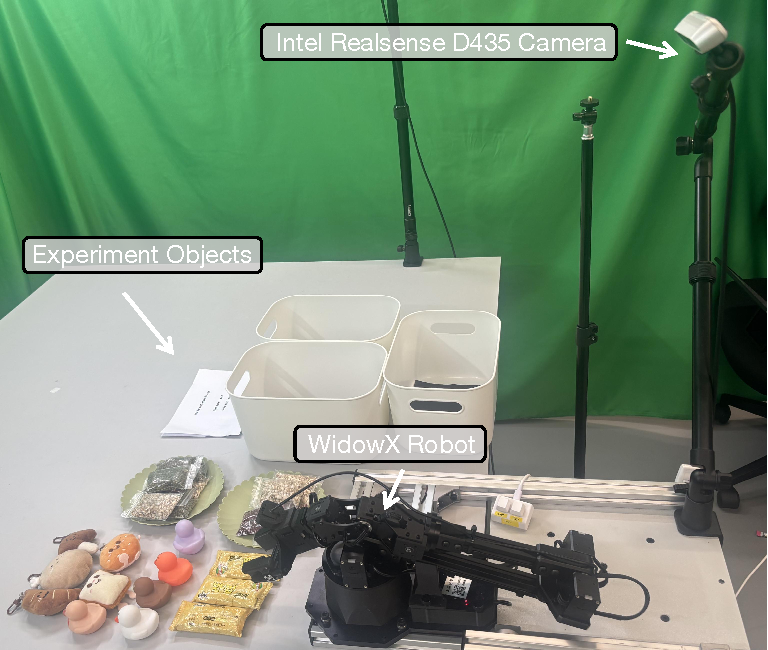
\includegraphics[width=0.9\linewidth]{imgs/setting.pdf}
    \caption{Real-world experimental setup. The system consists of a WidowX-250 robot arm, a front-facing Intel RealSense D435 camera, and a tabletop workspace containing task objects and storage boxes.}
    \label{fig:real_robot_setup}
\end{figure}

During data collection, both the external camera and the wrist camera record RGB observations at 25\,Hz. Each trajectory is synchronized with robot proprioceptive states, including end-effector pose, joint states, and gripper state. After collection, raw trajectories are processed through a standardized preprocessing pipeline. All images are resized to $224 \times 224$, and the trajectories are temporally subsampled to 10\,Hz. The processed demonstrations are then converted into the LeRobot format for downstream training.


\section{Analysis of Sentry's Working Memory and Termination Policy}


\begin{figure}[h]
    \centering
    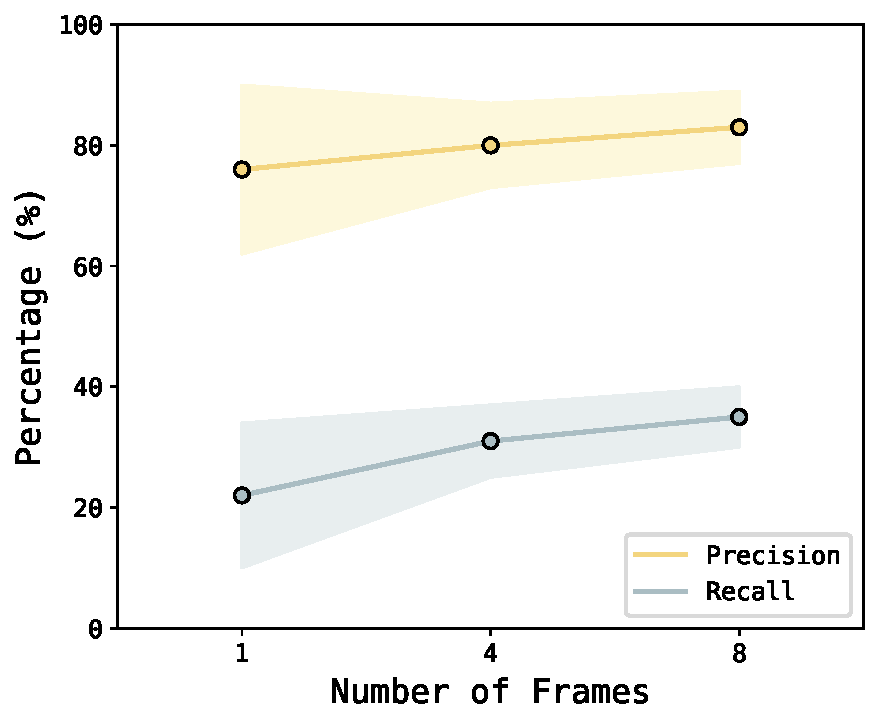
\includegraphics[width=.5\linewidth]{imgs/window_sentry.pdf}
    \caption{Increasing the number of recent frames provided to the Sentry leads to a consistent improvement in both precision and recall. This indicates that a longer temporal context is beneficial for accurate subtask monitoring.}
    \label{fig:sentry_ablation}
\end{figure}

To understand the Sentry's decision-making boundary, we analyzed its performance on subtask completion detection under different working memory sizes (window length $N$). \autoref{fig:sentry_ablation} presents the Precision and Recall, where Subtask ``Done'' is treated as the positive class.

% \siyin{standardize the scale and all use percentages.}
\textit{1) Benefits of Temporal Context:}
As shown in the \autoref{fig:sentry_ablation}, increasing the context window from 1 to 8 frames improves both Precision (from $\sim76\%$ to $\sim82\%$) and Recall (from $\sim22\%$ to $\sim35\%$).
A single frame often lacks sufficient information to distinguish between a temporary pause and true completion.
By observing a sequence of 8 frames (consistent with our sentry‘s working memory), the Sentry can leverage temporal cues to make more reliable judgments.

\textit{2) The "Conservative" Nature of Sentry:}
The significant gap between high Precision and low Recall reveals the Sentry's inherent ``conservative'' nature.
The system exhibits a strong bias towards the incomplete state, preferring to continue execution unless overwhelmingly confident that the goal is met.
While this minimizes premature stops (high Precision), the low Recall creates a ``missing signal'' problem where the agent might overshoot its target or enter infinite loops.
Since the Sentry is prone to False Negatives (missing the ``Done'' event), we design a fixed-interval Planner fallback.It ensures that execution loops are eventually broken even when the Sentry fails to trigger.

\section{Additional Experiments}
\label{sec:additional_experiments}

We provide additional experiments to further analyze controlled memory management, planner generalization with open-source VLMs, memory scalability over extended horizons, and system latency.

\subsection{Controlled Memory Ablation}
\label{sec:controlled_memory_ablation}

We first conduct a controlled memory ablation on the \textbf{Rearrangement} task to separate the effect of memory management strategy from that of memory capacity. In the main setting, HiMe uses unconstrained active memory, while the FIFO baseline is evaluated with a fixed memory budget. Although the FIFO budget is chosen to match the average memory size of the unlimited active baseline, the two settings still differ in whether memory is explicitly constrained. To provide a cleaner comparison, we additionally evaluate a limited-memory version of active management under the same fixed budget.

Specifically, we compare three variants: \textbf{Unlimited Active Management}, corresponding to the original HiMe setting with unconstrained memory; \textbf{Limited Active Management}, which uses the same Add / Update / Delete mechanism under a fixed budget of 8 entries; and \textbf{FIFO (Limited)}, which uses the same budget with FIFO eviction.

\begin{table}[H]
\centering
\caption{Controlled memory in Rearrangement.}
\label{tab:controlled_memory_ablation}
\begin{tabular}{lcc}
\toprule
\textbf{Method} & \textbf{Memory Budget} & \textbf{Task Progress (\%)} \\
\midrule
Unlimited Active Management & Unbounded & 87.0 \\
Limited Active Management & Fixed (8 entries) & 80.0 \\
FIFO (Limited) & Fixed (8 entries) & 64.0 \\
\bottomrule
\end{tabular}
\end{table}

Performance decreases under constrained memory, but active management remains substantially stronger than FIFO under the same capacity. This result indicates that the benefit of HiMe is not explained by larger memory alone, and that explicit Update / Delete operations remain useful beyond simple eviction.

\subsection{Open-Source Planner Evaluation}
\label{sec:opensource_planner_eval}

To improve reproducibility and examine planner generalization, we replace the main Planner with the open-source VLM \textbf{Qwen3-VL-30B} and evaluate the system on the \textbf{Rearrangement} task under the same protocol. The results are shown in Fig.~\ref{fig:qwen_appendix_more_exp}.

Fig.~\ref{fig:qwen_appendix_more_exp}(a) reports the main comparison with the corresponding baselines. Fig.~\ref{fig:qwen_appendix_more_exp}(b) presents the modality ablation, comparing the full system with text-only and image-only memory. Fig.~\ref{fig:qwen_appendix_more_exp}(c) shows the memory ablation under the same open-source Planner. Overall, the trends are consistent with the main experiments: HiMe remains the best-performing variant with Qwen3-VL-30B, indicating that the benefits of structured memory and sentry-based coordination are robust to the choice of Planner.

\begin{figure}[H]
    \centering
    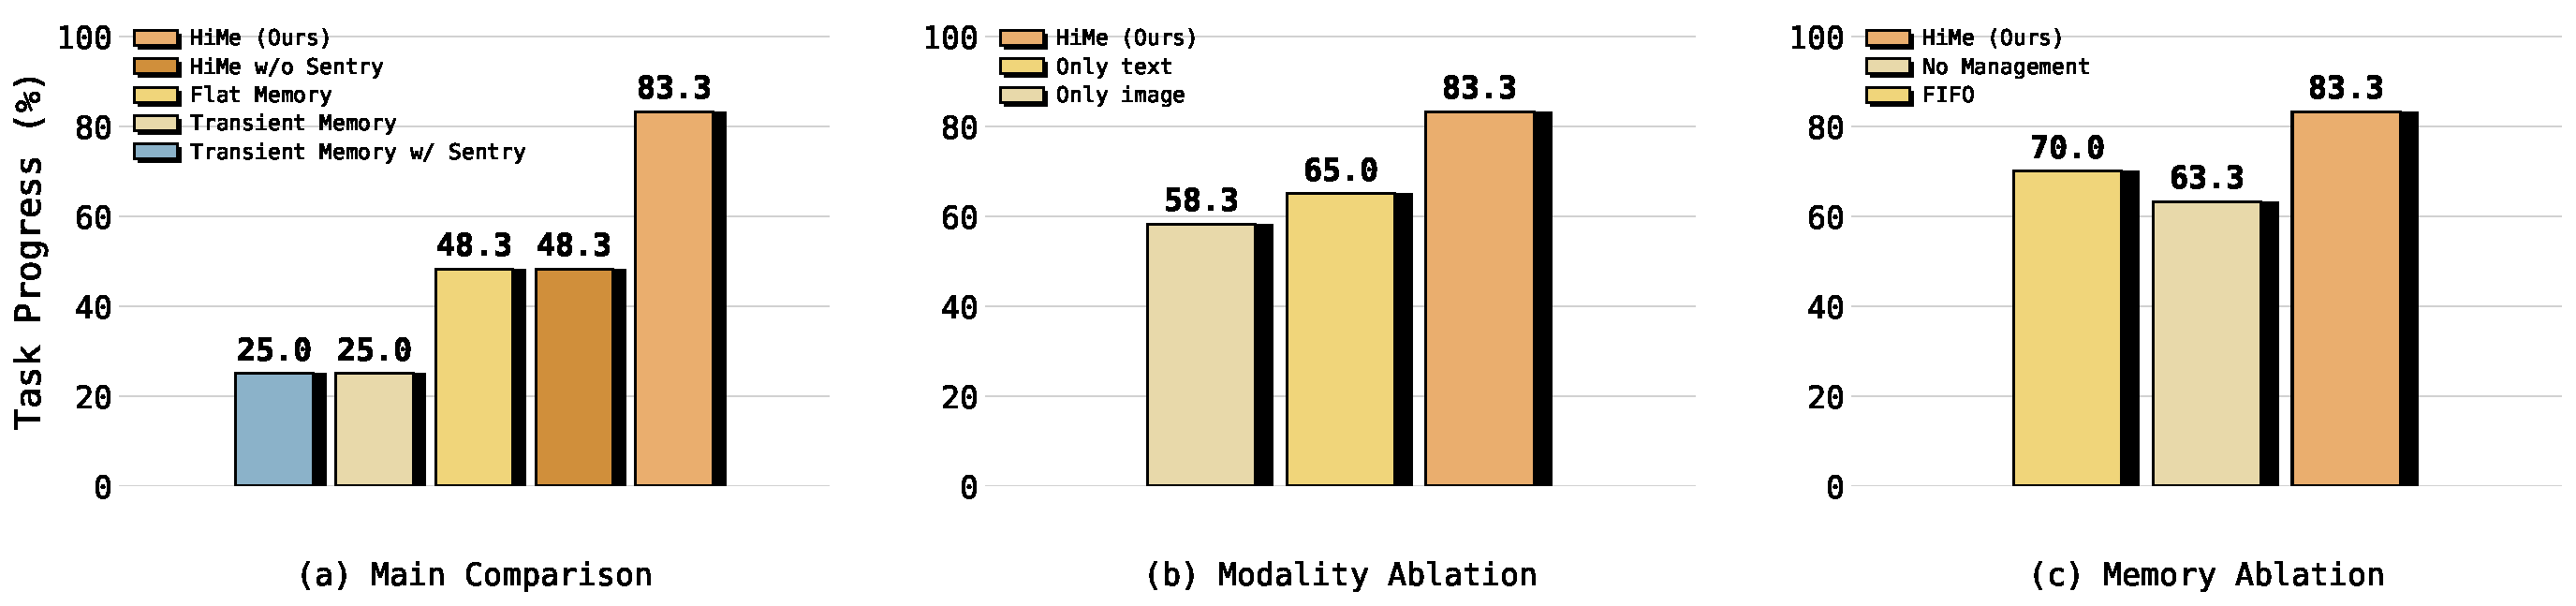
\includegraphics[width=\linewidth]{imgs/appendix_more_exp.pdf}
    \caption{Additional experiments on the \textbf{Rearrangement} task with \textbf{Qwen3-VL-30B} as the Planner. (a) Main comparison with the corresponding baselines. (b) Modality ablation. (c) Memory ablation. The overall trends are consistent with the main experiments, and HiMe remains the best-performing variant under the open-source Planner.}
    \label{fig:qwen_appendix_more_exp}
\end{figure}

\subsection{Memory Scalability}
\label{sec:memory_scalability}

We further analyze memory scalability using an extended multi-round version of \textbf{Object Search}. In each round, the robot must inspect boxes with initially unknown contents and place the visible table object accordingly. At the beginning of each new round, the box contents are changed, requiring the agent to re-inspect the scene and revise memory before acting. As the number of rounds increases, both the task horizon and the number of subtasks increase.

We report the average \textbf{Memory Size} and \textbf{Task Progress} across different numbers of rounds.

\begin{table}[H]
\centering
\caption{Memory scalability in extended multi-round Object Search.}
\label{tab:memory_scalability}
\begin{tabular}{cccc}
\toprule
\textbf{Rounds} & \textbf{Subtasks} & \textbf{Memory Size} & \textbf{Task Progress (\%)} \\
\midrule
1 & 4  & 5.5  & 92.5 \\
2 & 8  & 9.9  & 76.3 \\
3 & 12 & 14.0 & 66.7 \\
\bottomrule
\end{tabular}
\end{table}

As the horizon increases, memory size grows while task performance declines. This result suggests that the main challenge in long-horizon settings is not only storing more information, but also maintaining correct and up-to-date memory as the environment evolves.

\subsection{System Latency}
\label{sec:system_latency}

We additionally measure Planner latency under different deployments. Each Planner call consists of two stages: memory query / retrieval, and plan generation together with memory update. We report end-to-end latency over complete Planner calls.

\begin{table}[H]
\centering
\caption{End-to-end Planner latency under different model deployments.}
\label{tab:system_latency}
\begin{tabular}{lcccc}
\toprule
\textbf{Model} & \textbf{P50 (s)} & \textbf{P90 (s)} & \textbf{P99 (s)} & \textbf{Avg. Completion Tokens} \\
\midrule
GPT-4o (API) & 38.59 & 49.30 & 57.28 & 517.9 \\
Qwen3-VL-30B (local) & 6.83 & 7.93 & 8.65 & 532.8 \\
Qwen3-VL-8B (local) & 6.10 & 7.08 & 11.34 & 399.0 \\
\bottomrule
\end{tabular}
\end{table}

Latency differences are mainly associated with deployment mode, i.e., remote API versus local serving, rather than token scale alone. In practice, HiMe is compatible with different planner backends, and local deployment substantially reduces reasoning latency. Since Planner calls are triggered only when necessary, this reasoning latency remains decoupled from the high-frequency low-level control loop.

\newpage
\section{Prompts Details}

\begin{tcolorbox}[colback=black!2, colframe=black!45, title=Sentry Prompt]
You are the \textbf{EXECUTION OBSERVER} of an embodied agent.

\textbf{Primary input modality:}
\begin{itemize}[leftmargin=*]
    \item \textbf{Plan list:}
    \begin{itemize}
        \item The model’s current decomposition of the task into subtasks.
        \item Each subtask line includes its execution status (e.g., [done], [current], [pending]).
    \end{itemize}
    
    \item \textbf{Combined images of recent frames:}
    \begin{itemize}
        \item \textbf{CRITICAL LAYOUT INFO:} Each image is a composite.
        \item LEFT HALF: Wrist Camera View (Close-up, attached to the gripper).
        \item RIGHT HALF: Third-Person View (Global view of the robot and environment).
    \end{itemize}
\end{itemize}

Your \textbf{ONLY} job is to judge whether the \textbf{CURRENT} subtask has been completed.

\textbf{Judgment Criteria:}
\begin{itemize}[leftmargin=*]
    \item \textbf{Inspect:} done when the robot arm is above or extended into the box, and the wrist view shows the content and the black background of the box.
    
    \item \textbf{Pick \& Place:} done when the object has been successfully released at the destination or you observe that the robot arm is above a box and see its black background.
    
    \item \textbf{Reset:} done when the robot arm is in the home pose.
    \begin{itemize}
        \item The robot arm home pose is: in both images, the arm is aligned parallel to what appears to be a rail or track. The end effector (or gripper) is open and facing downwards towards the table.
    \end{itemize}
    
    \item The interior bottom surface of the box is lined with a black background to enhance contrast for detection.
\end{itemize}

\noindent\rule{\linewidth}{0.4pt} % 分割线

\textbf{\# REQUIRED OUTPUT FORMAT}

You \textbf{MUST} output exactly this XML structure:

\begin{verbatim}
<status>
<!-- EXACTLY one of:
        done
        not_done
-->
</status>
\end{verbatim}

\end{tcolorbox}

\begin{tcolorbox}[
    enhanced,                   % 启用增强绘图引擎（修复渲染问题）
    colback=white,              % 强制背景为纯白 (如果觉得太亮，可改为 black!5)
    colframe=blue!50!black,     % 边框颜色：深蓝
    coltext=black,              % 强制文字为黑色
    title=Planner Prompt,
    fonttitle=\bfseries,        % 标题加粗
    breakable,                  % 允许跨页
    arc=2mm                     % 圆角大小
]

You are the \textbf{PLANNER} of an embodied agent.

\textbf{Primary input modalities:}
\begin{itemize}[leftmargin=*]
    \item \textbf{User instruction:} The user's high-level instruction for the agent.
    \item \textbf{Plan list:} The model's current decomposition of the task into subtasks. Each subtask line includes its execution status (e.g., [done], [current], [pending]).
    \item \textbf{Combined images during subtask execution:}
    \begin{itemize}
        \item \textbf{IMAGE LAYOUT \& USAGE GUIDE:}
        \item \textbf{LEFT HALF (Wrist View):} Egocentric view attached to the gripper. Usage: Identify specific objects, read text, verify grasping.
        \item \textbf{RIGHT HALF (Third-Person View):} Global view. Usage: Spatial context, locating containers, tracking arm position.
        \item \textbf{NOTE:} Integrate information from both. Use Right view to navigate, Left view to inspect.
    \end{itemize}
\end{itemize}

You have access to an external \textbf{MEMORY} module through a structured CRUD interface.
MEMORY stores records with fields: \texttt{id}, \texttt{tags}, \texttt{data} (type, value), \texttt{image\_path}.

\noindent\rule{\linewidth}{0.4pt}

\textbf{\# TAG DESIGN PRINCIPLES}

Tags are the PRIMARY mechanism for memory retrieval.

\begin{enumerate}[leftmargin=*]
    \item \textbf{OBJECT TAGS:} \texttt{toy\_duck}, \texttt{snack\_package}, \texttt{left\_box}.
    \item \textbf{LOCATION TAGS:} \texttt{table}, \texttt{shelf}, \texttt{inside\_left\_box}.
    \item \textbf{USER\_PREFERENCE TAGS:} \texttt{user}, \texttt{lily}, \texttt{likes}, \texttt{prefers}.
\end{enumerate}

\textbf{Tag Usage Rules:} Use 2-5 tags per record. Update tags when object state changes.
\textbf{Tag Query Strategy:} PREFER tag-based queries. Query one tag every time.

\noindent\rule{\linewidth}{0.4pt}

\textbf{\# MEMORY CRUD PROTOCOL}

You interact with memory only via structured XML operations.

\textbf{(1) QUERY (READ)}
\begin{verbatim}
<operation>
  <type>QUERY</type>
  <query>search key tags</query>
  <reason>why you search this</reason>
</operation>
\end{verbatim}

\textbf{(2) CREATE}
\begin{verbatim}
<operation>
  <type>CREATE</type>
  <tags>...</tags>
  <text>concise description or fact</text>
  <image_path>index</image_path>
  <reason>why this new memory is necessary</reason>
</operation>
\end{verbatim}

\textbf{(3) UPDATE}
\begin{verbatim}
<operation>
  <type>UPDATE</type>
  <id>record_id</id>
  <tags>...</tags>
  <text>updated description</text>
  <image_path>2</image_path>
  <reason>why this existing record must be changed</reason>
</operation>
\end{verbatim}

\textbf{(4) DELETE}
\begin{verbatim}
<operation>
  <type>DELETE</type>
  <id>...</id>
  <reason>why this record is no longer useful</reason>
</operation>
\end{verbatim}

\noindent\rule{\linewidth}{0.4pt}

\textbf{\# EVIDENCE RELIABILITY RULES (NO ASSUMPTIONS)}
\begin{itemize}[leftmargin=*]
    \item Memory must contain only verifiable facts derived from explicit user instructions or direct visual evidence.
    \item \textbf{Do NOT CREATE FAKE memory.} Prefer planning an inspection step.
    \item UPDATE is for correcting/refining without changing time meaning.
    \item When state changes, \textbf{CREATE} a new record, UPDATE the old one to label as past.
    \item DELETE sparingly (only for duplicates or errors).
\end{itemize}

\noindent\rule{\linewidth}{0.4pt}

\textbf{\# MEMORY USAGE POLICY (TWO-TURN INTERACTION)}
\begin{itemize}[leftmargin=*]
    \item \textbf{Turn 1 (QUERY-only):} Issue QUERY operations. NO Create/Update/Delete. Plan list must be empty.
    \item \textbf{Turn 2 (REFINE + CRUD):} Issue Create/Update/Delete based on query results. Output finalized \texttt{<plan\_list>}.
\end{itemize}

\noindent\rule{\linewidth}{0.4pt}

\textbf{\# PLAN LIST FORMAT (FINAL OUTPUT ONLY, TURN 2)}
Plain text, one subtask per line.
\begin{itemize}
    \item \texttt{[done]}: subtask completed.
    \item \texttt{[current]}: the single subtask to execute NEXT.
    \item \texttt{[pending]}: future subtasks.
\end{itemize}
Annotation: You MAY include a short purpose in parentheses, e.g., \texttt{[pending] inspect recipe (check what does it need)}.

\noindent\rule{\linewidth}{0.4pt}

\textbf{\# PLAN LIST ACTION FORMAT}
\begin{enumerate}[leftmargin=*]
    \item \textbf{Inspection action:} Main verb "inspect". Use when information is missing.
    \item \textbf{Pick-and-place action:} "pick up \texttt{<object>} \texttt{<source>} and place it to \texttt{<target>}".
\end{enumerate}

\noindent\rule{\linewidth}{0.4pt}

\textbf{\# REQUIRED OUTPUT FORMAT FOR EACH TURN}

\begin{verbatim}
<summary>
  <!-- Concise reasoning summarizing observations and memory interaction -->
</summary>

<memory_operations>
  <!-- Turn 1: QUERY only. Turn 2: CRUD operations. -->
</memory_operations>

<plan_list>
  <!-- Turn 1: EMPTY.
       Turn 2: Finalized plan list.
       [done] ...
       [current] ...
       [pending] ...
  -->
</plan_list>
\end{verbatim}

\end{tcolorbox}





% \section{Case Study}
% memory content





